\titleformat{\chapter}[display]
{\normalfont\huge\bfseries}{Capítulo \thechapter}{0.5em}{\huge}
\titlespacing*{\chapter}{0pt}{-1.25cm}{25pt}
\chapter{Introducción}
\section{Arritmias}
Las enfermedades cardiovasculares son la primera causa de muerte en el mundo y una de las causas mas comunes
de estas enfermedades son las arritmias.

Una arritmia cardiaca es una alteración en el ritmo normal del corazón. Si se produce una arritmia, el corazón 
puede latir demasiado rápido, demasiado lento o de manera irregular. Esto puede provocar síntomas como palpitaciones,
mareos, falta de aire e incluso desmayos y estas pueden llegar a ser mortales.

Los cardiologos utilizan dispositivos como un Holter para generar tiras de ritmo o electrocardiogramas, que es un 
diagrama que representa los latidos del corazon y con eso pueden llegar a detectar arritmias.

\begin{figure}[h!]
	\centering
	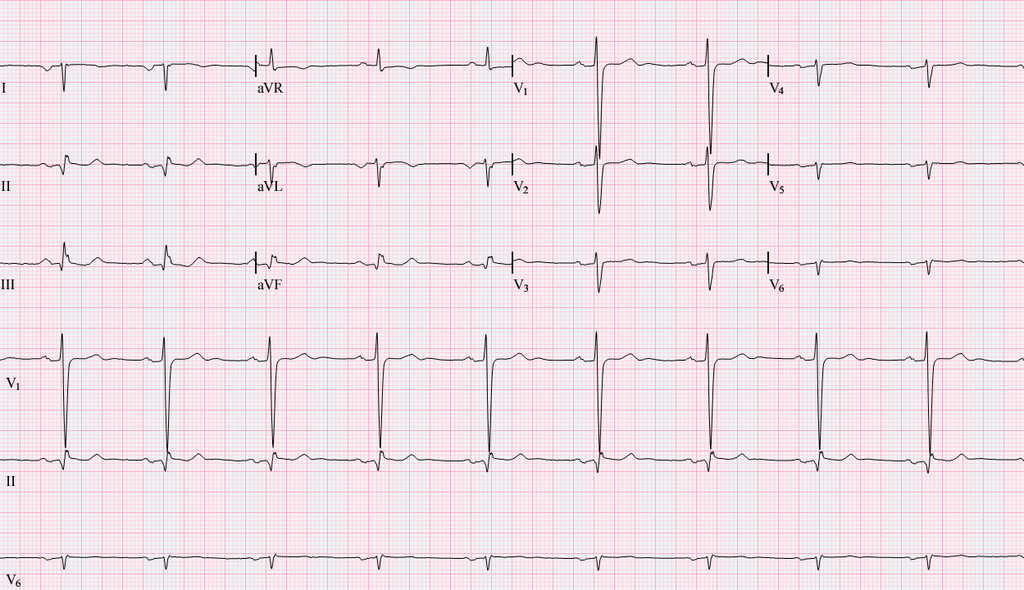
\includegraphics[width=0.7\textwidth]{./Images/img_introduccion/electrocardiograma.png}
	\caption{Electrocardiogramas}
	\label{fig:electrocardiogramas}
\end{figure}

En este proyecto se tratara de solucionar las arritmias en las que se produce una contraccion prematura del corazon
como las contracciones prematuras del corazón. Estas arritmias se 
pueden detectar con un electrocardiograma (ECG) que es un diagrama de los latidos del corazon.



\section{Algoritmo de deteccion}
Dado que para detectar arritmias correctamente se necesitan varios años de cardiologia,el algoritmo de 
deteccion que se utilizara consistira en detectar las arritmias unicamente usando los picos QRS del electrocardiograma.

Un pico QRS como se muestra en la \Cref{fig:complejoQRS} en un electrocardiograma es causado por la contaccion del ventriculo al bombear la sangre por las arterias.
Este es el impulso electrico mas fuerte que el corazon produce en cada latido. En este proyecto utilizaremos estos picos
para comparar la distancia entre ellos y poder ver si se ha producido una arritmia. 

\begin{figure}[h]
	\centering
	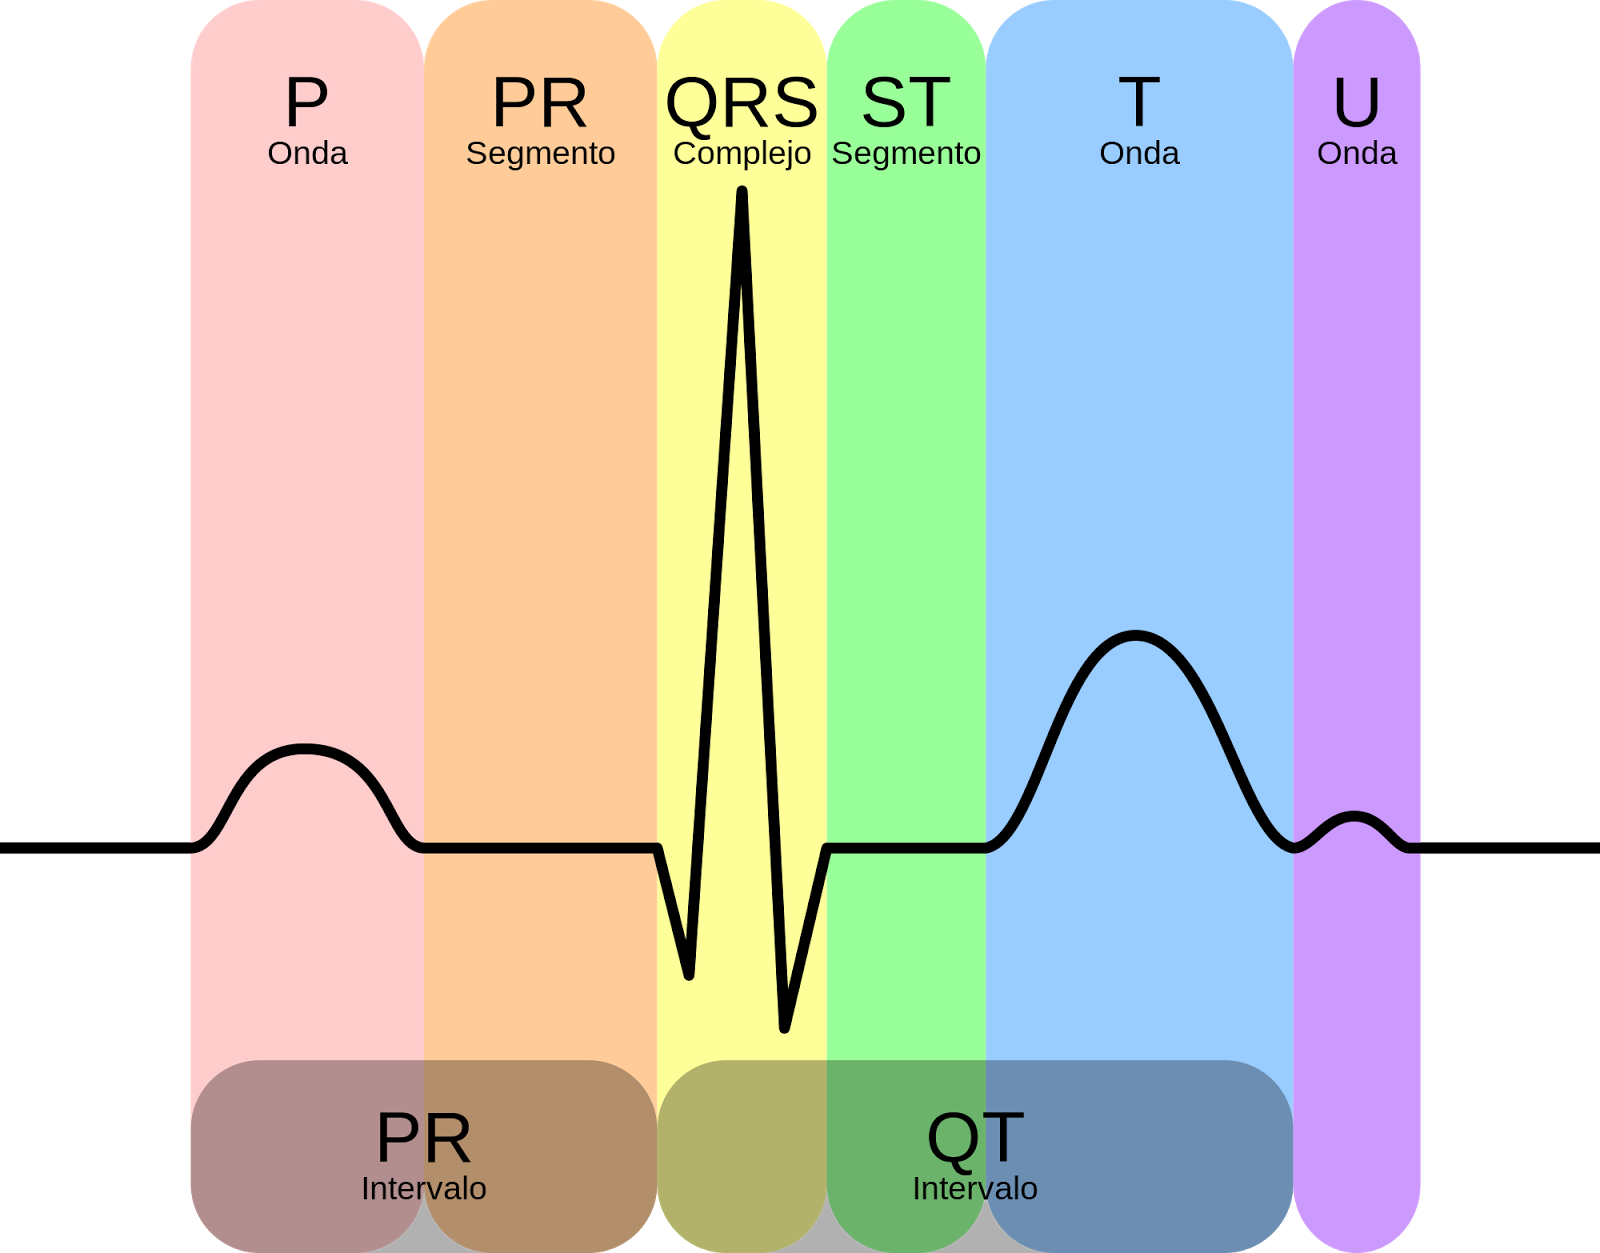
\includegraphics[width=0.4\textwidth]{./Images/img_introduccion/complejoQRS.png}
	\caption{Complejo QRS}
	\label{fig:complejoQRS}
\end{figure}

\subsection{Filtrado}
Como se puede ver en las imagenes es conveniente hacer un filtrado de las tiras de ritmo para poder detectar mejor
los picos QRS. Ya que el filtrado centra la onda en el 0 y evita fallos en el algoritmo de deteccion de picos del 
que se hablará mas adelante. 

En la creacion del proyecto se ha intentado no filtrar la onda para comprobar si se obtienen mejores resultados que
sin dicho filtrado pero no se ha dado el caso por las irregularidades de la misma.

\begin{figure}[h!]
	\centering
	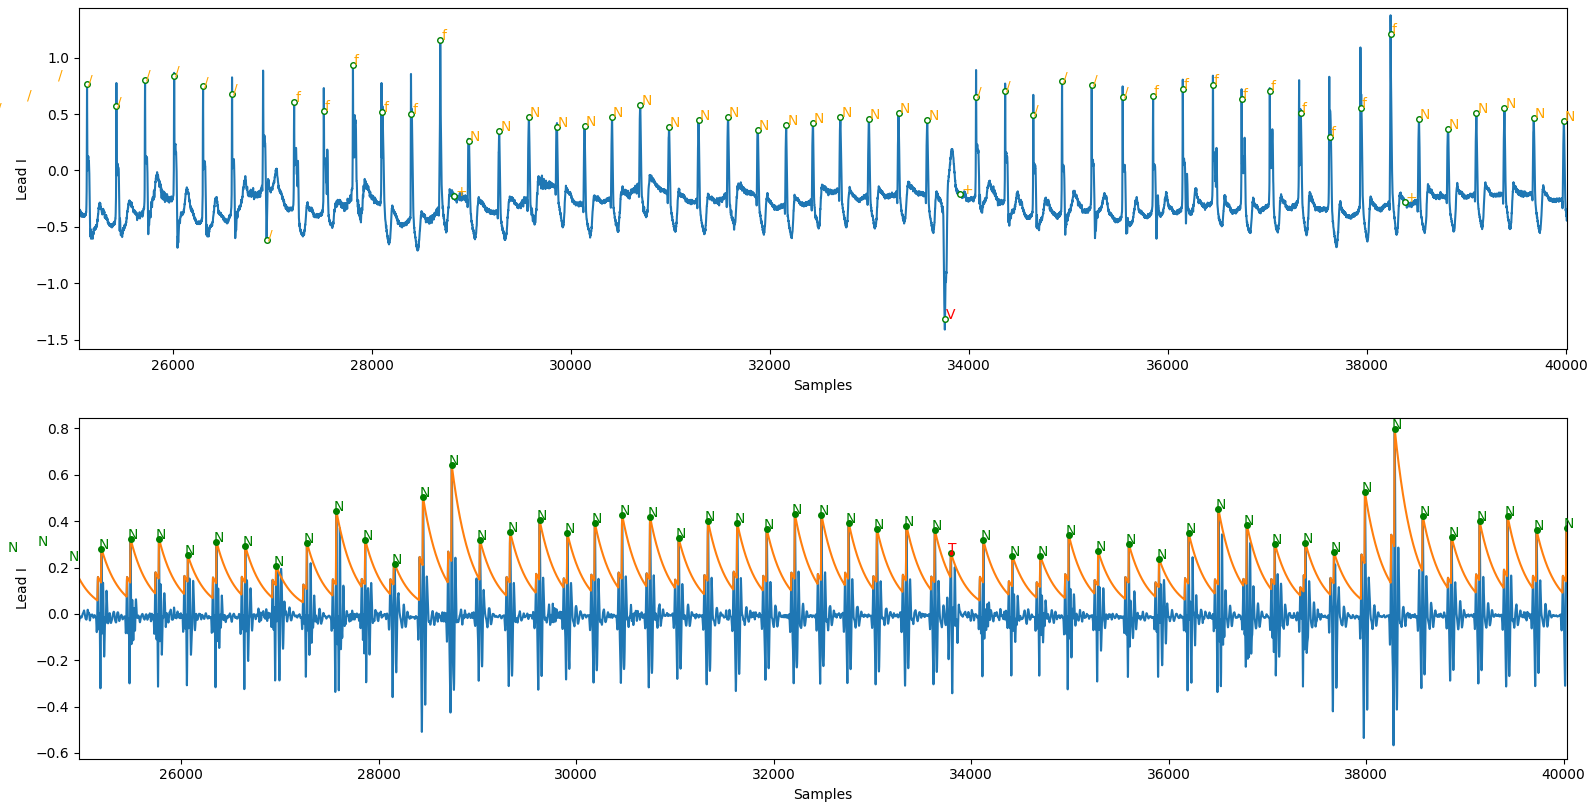
\includegraphics[width=0.99\textwidth]{./Images/img_introduccion/102filtrado_y_sin_filtrar.png}
	\caption{Ejemplo de electrocardiograma original y filtrado de paciente 102}
	\label{fig:102filtradoysinfiltrar}
\end{figure}

\section{Pruebas con pacientes}
Se han realizado las pruebas con unos resultados del Instituto de Tecnología de Massachusetts (MIT) en el que se han
recogido tiras de ritmo de media hora de varios pacientes con edades diversas y algunos de ellos llevan un marcapasos
que actua cuando el corazón no bombea la sangre lo suficientemente fuerte, es decir que el pico QRS no es tan prominente
y se necesita la ayuda de dicho marcapasos para proporcionar el impulso electrico necesario.

Estas pruebas han sido analizadas por cardiologos y se ha indicado donde el paciente padece una arritmia y donde el ritmo
es normal y donde se ha producido un error en la lectura de la señal. Tambien muestra informacion menos relevante como la 
activacion del marcapasos.

\begin{figure}[h]
	\centering
	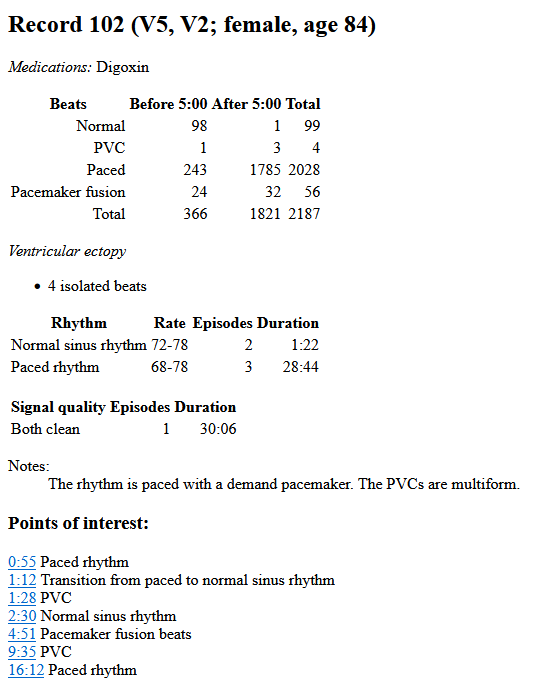
\includegraphics[width=0.6\textwidth]{./Images/img_introduccion/Paciente_pruebas_MIT.png}
	\caption{Ejemplo con paciente 102}
	\label{fig:Paciente_pruebas_MIT}
\end{figure}

\section{Utilizacion de las FPGAs}
Este proyecto requiere un gran procesamiento de señales, una alta cantidad de calculos y un eficiente paralelismo 
entre modulos por ello la mejor forma de optimizar el algoritmo es utilizando una FPGA.

Los motivos son los siguientes:

\begin{itemize}
	\item Las FPGA pueden procesar datos a velocidades muy altas, lo que lo hace indispensable para esta aplicacion
	 que esta pensada para ejecutarse en tiempo real.
	\item Las FPGA son dispositivos de hardware programable que permite diseñar circuitos digitales personalizados, 
	y por ello pueden reconfigurarse para adaptarse a tareas específicas. Ademas son susceptibles a cambios en el 
	algoritmo para una posible mejora de este.
	\item El alto paralelismo que ofrecen las FPGA es perfecto para las multitareas que realiza el algoritmo.
	\item Puesto que las FPGA pueden ser diseñadas para realizar una tarea en concreto, estas son mas energeticamente
	eficientes que otros dispositivos como los portatiles.
\end{itemize}

Para este proyecto se usara la FPGA Basys3 de Artix-7 para probar el funcionamiento del algoritmo. Aunque se debe considerar, segun
la cantidad de datos introducidos, que en este caso seria la longitud de la señal segun el tiempo transcurrido, utilizar
una FPGA cuyo hardware pueda soportar dicha cantidad de datos.


\section{Objetivos del proyecto y organización}
Los objetivos de este proyecto es tener una solucion para detectar contracciones prematuras ventriculares a tiempo real en
un largo periodo de tiempo y optimizar el algoritmo para que se ejecute de una forma mas eficiente y menos costosa en una FPGA

Para ello la organizacion de este proyecto comienza con la creacion de el prototipado del algoritmo en software para facilitar
la manera de probar el algoritmo con la solucion proporcionada por la base de datos y poder ver resultados graficos, para mejorar
la velocidad de compilacion y depuracion del algoritmo, para aumentar la claridad del algoritmo que se quiere conseguir en el
prototipado y para validar la funcionalidad y eficacia del algoritmo.
\section{Analisis y optimizacion del algoritmo}
Para lograr los objetivos del algoritmo se centra en tres funciones.
\begin{enumerate}
	\item Filtrado de la señal original: Lo que hace que la señal sea mas facil de procesar para encontrar los picos QRS.
	 Esto se realiza multiplicando los valores de la señal original por los valores de filtrado.
	\item Deteccion de picos sobre la señal filtrada: Se analiza cada señal y comparandola con otras señales anteriores se
	 deduce si puede ser un posible pico y si lo es, se comprueba si es un pico QRS.
	\item Deteccion de arritmias comparando la posicion de los picos: una vez se tienen los picos QRS se calcula la distancia
	 de el pico actual con el pico anterior y dependiendo de las otras distancias se calcula si hay una arritmia.
\end{enumerate}


\section{Implementacion en la FPGA}
Para implementar el codigo en la FPGA se implementaran varios modulos para tratar de imitar el proyecto creado en software 
los modulos mas importantes son.

	\begin{enumerate}
		\item Modulo de filtrado: Se guardan los valores del filtrado en una memoria y se van multiplicando los valores que van llegando 
		al modulo. estos valores multiplicados a su vez se almacenan en memoria hasta que pasan al siguente módulo
		\item Deteccion de picos sobre la señal filtrada: Se analiza cada señal que pasa del modulo de filtrado y mediante una maquina de estados
		se busca el pico mas alto dentro de los limites del cutoff, si se encuentra se comprueba si es un pico QRS.
		\item Deteccion de arritmias comparando la posicion de los picos: una vez se tienen los picos QRS se implementa una maquina de estados que
		sea capaz de hallar la distancia entre 2 picos, meterla en un buffer y calcular el porcentaje de el tamaño de la distancia con las demas.
	\end{enumerate}

	Estos modulos tratan de replicar las funcionalidades que realiza el algoritmo de software y se convertiran en la parte esencial
	de dicho programa. 
	
	Además de estos modulos se debe de crear un modulo que acompase a estos tres y un testbench para probar el funcionamiento
	del programa en la simulación.